\section{Introduction}

\subsection{Compressor Systems}

\begin{frame}{Compressor Systems}
  \begin{itemize}
    \item Used often in natural gas installations
    \item Very energy-intensive process
      \begin{itemize}
        \item Small improvements in efficiency $\implies$ large energy/capital savings
      \end{itemize}
    \item Complex system from control perspective
      \begin{itemize}
        \item Highly non-linear
        \item Multivariable, highly coupled
        \item Hard input constraints and rate constraints
        \item Unstable regimes (surge, stall)
      \end{itemize}
    \item Highest efficiencies often near surge line
  \end{itemize}

  \vfill
  \pause
  \alert{\centering Increasing control performance can significantly reduce costs\\}
\end{frame}

\subsection{Conventional Control}
\begin{frame}{Conventional Control}
  % What does conventional control look like?\\
  % What are the upsides?\\
  % What are the downsides?\\
  % What are the things that are fundamentally impossible to treat?
  \centering
  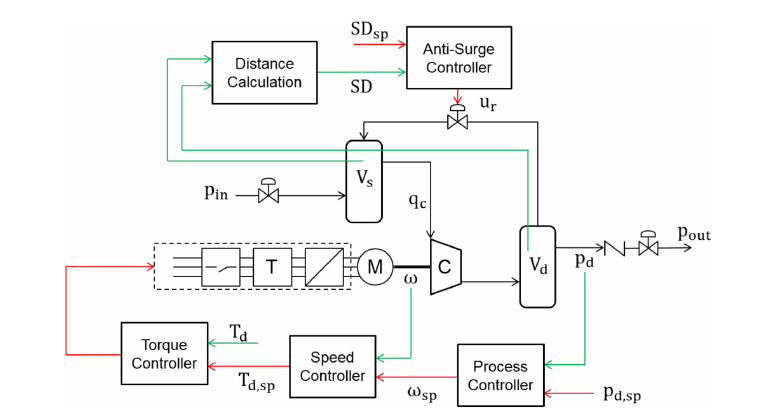
\includegraphics[width=0.7\linewidth]{intro/diagram.png}
  \begin{itemize}
    \item Separate process and anti-surge controllers (ASC)
    \item Loop decoupling and anti-windup terms
    \item Potential of electric drivers not fully utilized
    % \item \alert{Constraints and coupling not treated directly}
  \end{itemize}
  \alert{Potential for increased performance with multivariable control}
\end{frame}

\subsection{MPC Approaches}
\begin{frame}{Model Predictive Control}

  {\usebeamercolor[fg]{structure}\bfseries Advantages:\\}
  \begin{itemize}
    \item Combine process control and ASC
    \item Use fast response of electric drivers to improve ASC performance
    \item Treat constraints explicitly
  \end{itemize}
  \vspace{1em}
  {\usebeamercolor[fg]{structure}\bfseries Disadvantages:\\}
  \begin{itemize}
    \item Increased computation time -- especially for large systems
    \item Centralized control $\implies$ difficult to implement in industrial setting
  \end{itemize}
  \vspace{1em}

  \pause

  {\centering
    \alert{Use distributed MPC to decrease computation time}\\
  }

  % What advantages can MPC offer?\\
  % What has already been proven with MPC?\\
  % Why is MPC better?\\
  % What are its disadvantages?
\end{frame}

\begin{frame}{Overview}
  \begin{multicols}{2}
    \tableofcontents[%currentsection,
    %currentsubsection,
  subsectionstyle=shaded/shaded/show,
sectionstyle=shaded/show]
  \end{multicols}
\end{frame}

